% Memory hierarchy as a pyramid. Higher levels are smaller and faster.
% The sizes and latencies are typical orders of magnitude for a current server CPU.
% Replace them with the values of your machine.
\documentclass[border=5pt]{standalone}
\usepackage{tikz}
\usetikzlibrary{calc}
\begin{document}
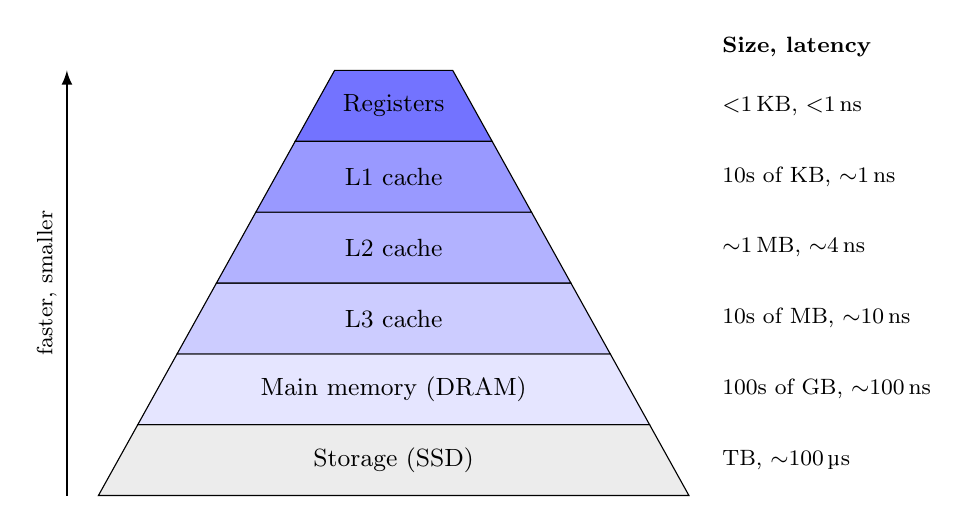
\begin{tikzpicture}[
    level/.style={font=\small},
    note/.style={font=\footnotesize, anchor=west, align=left},
]
\def\H{0.9}   % height of one level
\def\W{7.5}   % width of the base
\def\N{6}     % number of levels
% level index, label, fill, size, latency
\foreach \i/\name/\col/\size/\lat in {
    0/Storage (SSD)/gray!15/{TB}/{$\sim$100\,\textmu s},
    1/Main memory (DRAM)/blue!10/{100s of GB}/{$\sim$100\,ns},
    2/L3 cache/blue!20/{10s of MB}/{$\sim$10\,ns},
    3/L2 cache/blue!30/{$\sim$1\,MB}/{$\sim$4\,ns},
    4/L1 cache/blue!40/{10s of KB}/{$\sim$1\,ns},
    5/Registers/blue!55/{$<$1\,KB}/{$<$1\,ns}} {
    \pgfmathsetmacro{\yb}{\i*\H}
    \pgfmathsetmacro{\yt}{(\i+1)*\H}
    % The denominator \N+1.5 leaves a flat top wide enough for the top label.
    \pgfmathsetmacro{\xbl}{\W/2*\i/(\N+1.5)}
    \pgfmathsetmacro{\xtl}{\W/2*(\i+1)/(\N+1.5)}
    \filldraw[fill=\col, draw=black] (\xbl,\yb) -- (\W-\xbl,\yb) -- (\W-\xtl,\yt) -- (\xtl,\yt) -- cycle;
    \node[level] at (\W/2, \yb+\H/2) {\name};
    \node[note] at (\W+0.3, \yb+\H/2) {\size, \lat};
}
% Axis arrows on the left
\draw[-latex, thick] (-0.4,0) -- (-0.4,\N*\H) node[midway, above, rotate=90, font=\footnotesize] {faster, smaller};
\node[note, font=\footnotesize\bfseries] at (\W+0.3, \N*\H+0.3) {Size, latency};
\end{tikzpicture}
\end{document}
